\section{Results and Discussion}

\begin{figure*}%[!htbp]

\begin{center}
\setlength\tabcolsep{1.5pt} % default value: 6pt
\begin{tabular}{ | c || c c c | c c c | c | c | }
  \multicolumn{8}{c}{} & \multicolumn{1}{c}{Control} \\
  \multicolumn{1}{c}{} & \multicolumn{3}{c}{Competitors} & \multicolumn{3}{c}{Mean Dominant ($\pm S.D.$)} & \multicolumn{1}{c}{ Pop Mean ($\pm S.D.$)} & \multicolumn{1}{c}{ Pop Mean ($\pm S.D.$)} \\
 \cline{2-9}
  \multicolumn{1}{c|}{} & \tiny{$P_{1} = 1.0$} & \tiny{$P_{2} = P_{1}$} & \tiny{$P_{2} > P_{1}$} & \tiny{$P_{1} = 1.0$} & \tiny{$1.0 > P_{1} > P_{2}$} & \tiny{$P_{2} \geq P_{1}$} & \tiny{\textit{all}} & \tiny{\textit{all}}  \\
 \hline
 $Upd.$ & 25M & 25M & 25M & 25M & 25M & 25M & 200k & 200k \\
 $n$ & 1 & 1 & 1 & 9 & 7 & 34 & 50 & 50 \\
 \hhline{|=||===|===|=|=|}
 $A_1$ & 0.00 & 0.00 & 0.89 & $0.23 \pm 0.35$ & $0.50 \pm 0.47$ & $0.57 \pm 0.46$ & $0.51 \pm 0.14$ & $0.46 \pm 0.30$\\
 $A_2$ & 1.00 & 1.00 & 1.00 & $1.00 \pm  0.00$ & $1.00 \pm 0.00$ & $1.00 \pm 0.00$ & $1.00 \pm 0.00$ & $1.00 \pm 0.00$ \\
 \hline
 $P_{c}$ & 0.00 & 0.00 & 0.00 & $0.00 \pm 0.00$ & $0.00 \pm 0.00$ & $0.03 \pm 0.05$ & $0.07 \pm 0.03$ & $0.00 \pm 0.00$ \\
 $P_1$ & 1.00 & 0.50 & 0.00 & $1.00 \pm 0.00$ & $0.60 \pm 0.07$ & $0.28 \pm 0.16$ & $0.39 \pm 0.11$ & $0.04 \pm 0.08$ \\
 $P_2$ & 0.00 & 0.50 & 1.00 & $0.00 \pm 0.00$ & $0.40 \pm 007$ & $0.69 \pm 0.14$ & $0.54 \pm 0.11$ & $0.96 \pm 0.08$ \\
 \hline
 $C_1$ & 3.13 & 3.45 & 2.04 & $3.90 \pm 0.60$ & $3.38 \pm 0.33$ & $3.03 \pm 0.69$ & $3.38 \pm 0.23$ & $8.21 \pm 5.45$ \\
 $C_2$ & 233.2 & 238.6 & 290.2 & $230.6 \pm 71.1$ & $192.7 \pm 45.3$ & $271.6 \pm 73.6 $ & 99$.2 \pm 7.4 $& 350$.0 \pm 92.1 $ \\
 \hline
 $E_{c}$ & 0.87 & 0.14 & 4.20 & $0.29 \pm 0.37$ & $0.44 \pm 0.59$ & $0.21 \pm 0.75$ & $1.43 \pm 0.38$ & $2.77 \pm 1.50$ \\
 $E_1$ & 33.4 & 11.7 & 4.80 & $47.2 \pm 21.7$ & $21.3 \pm 12.0$ & $4.62 \pm 7.05$ & $31.5 \pm 6.6$ & $6.72 \pm 9.58$ \\
 $E_2$ & 341.4 & 397.4 & 321.1 & $231.2 \pm 94.3$ & $283.1 \pm 57.0$ & $325.4 \pm 68.9$ & $240.0 \pm 30.0$ & $317.5 \pm 55.2$ \\
 \hline
 $M_{c}$ & 0.11 & 1.00 & 0.66 & $0.33 \pm 0.41$ & $0.74 \pm 0.31$ & $0.67 \pm 0.35$ & $0.50 \pm 0.11$ & $0.20 \pm 0.23$ \\
 $M_1$ & 0.00 & 1.00 & 0.40 & $0.52 \pm 0.41$ & $0.65 \pm 0.46$ & $0.68 \pm 0.38$ & $0.50 \pm 0.12$ & $0.50 \pm 0.34$ \\
 $M_2$ & 0.00 & 0.44 & 1.00 & $0.45 \pm 0.39$ & $0.52 \pm 0.37$ & $0.50 \pm 0.42$ & $0.50 \pm 0.13$ & $0.50 \pm 0.33$ \\
 \hline
 $S_1$ & 0.00 & 1.00 & 1.00 & $0.65 \pm 0.38$ & $0.55 \pm 0.40$ & $0.47 \pm 0.42$ & $0.48 \pm 0.11$ & $0.48 \pm 0.34$ \\
 $S_2$ & 0.00 & 0.01 & 0.46 & $0.51 \pm 0.43$ & $0.35 \pm 0.39$ & $0.45 \pm 0.39$ & $0.49 \pm 0.13$ & $0.44 \pm 0.31$ \\
 \hline
\end{tabular}
\end{center}
\caption{
Enumerations for genotypes used as seeds for competition experiments (left) and enumerations for mean values of the most abundant genotype at the end of evolutionary runs (right), both sorted by resource-caching strategy.
}
\label{fig:genotypes}
\end{figure*}


\begin{figure*}%[!htbp]
\begin{center}
\thinmuskip=-2mu
\thickmuskip=-2mu
\nulldelimiterspace=-1pt
\scriptspace=0pt
\begin{subfigure}[b]{0.66\columnwidth}
  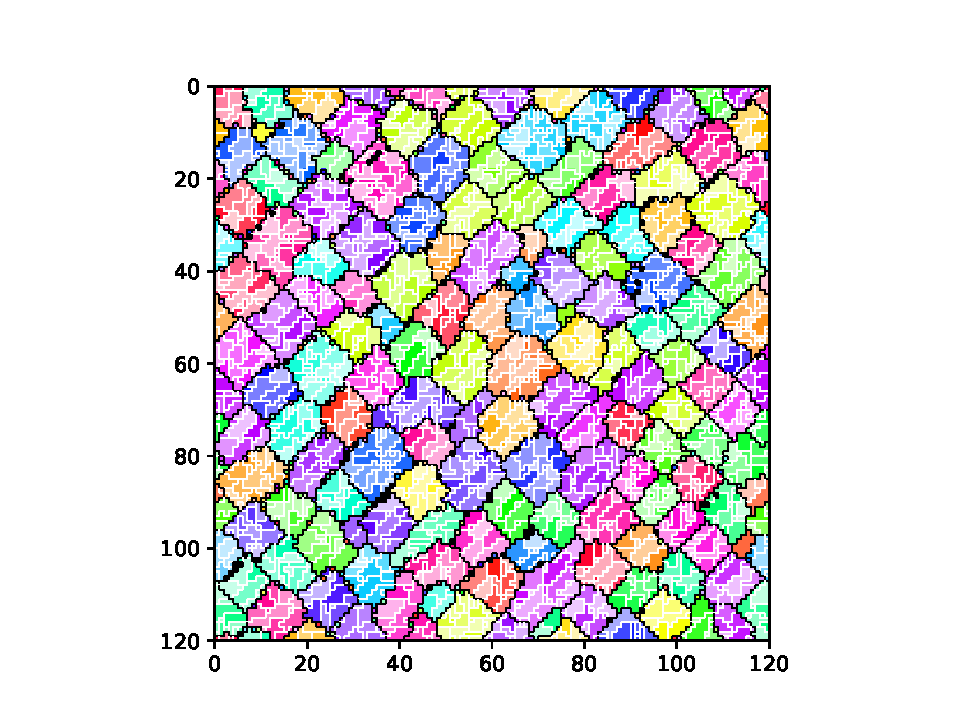
\includegraphics[width=\columnwidth,trim={2.5cm 0.5cm 2.5cm 1cm},clip]{img/ChannelMap_1022_update19500000}
  \caption{Mean $P_{c} = 0.77$, $P_1 = 0.09$, $P_2 = 0.14$; gen. 20,475}
  \label{fig:ChannelMap_1022}
\end{subfigure}%
\begin{subfigure}[b]{0.66\columnwidth}
  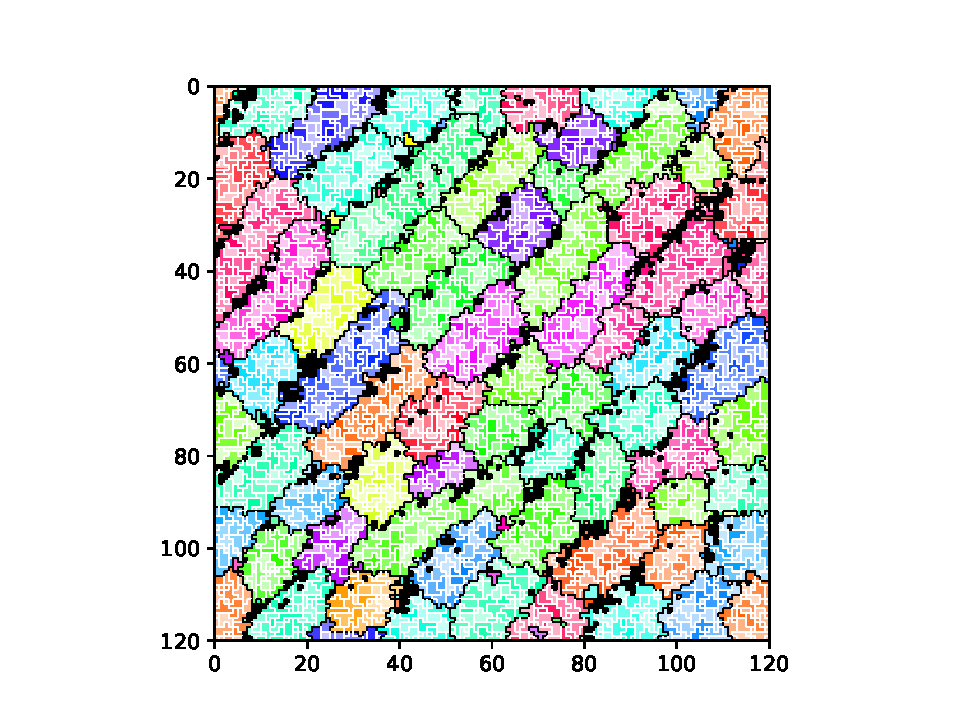
\includegraphics[width=\columnwidth,trim={2.5cm 0.5cm 2.5cm 1cm},clip]{img/ChannelMap_1041_update19500000}
  \caption{Mean $P_1 = 1.0$; gen. 23,971\\~}
  \label{fig:ChannelMap_1041}
\end{subfigure}%
\begin{subfigure}[b]{0.66\columnwidth}
  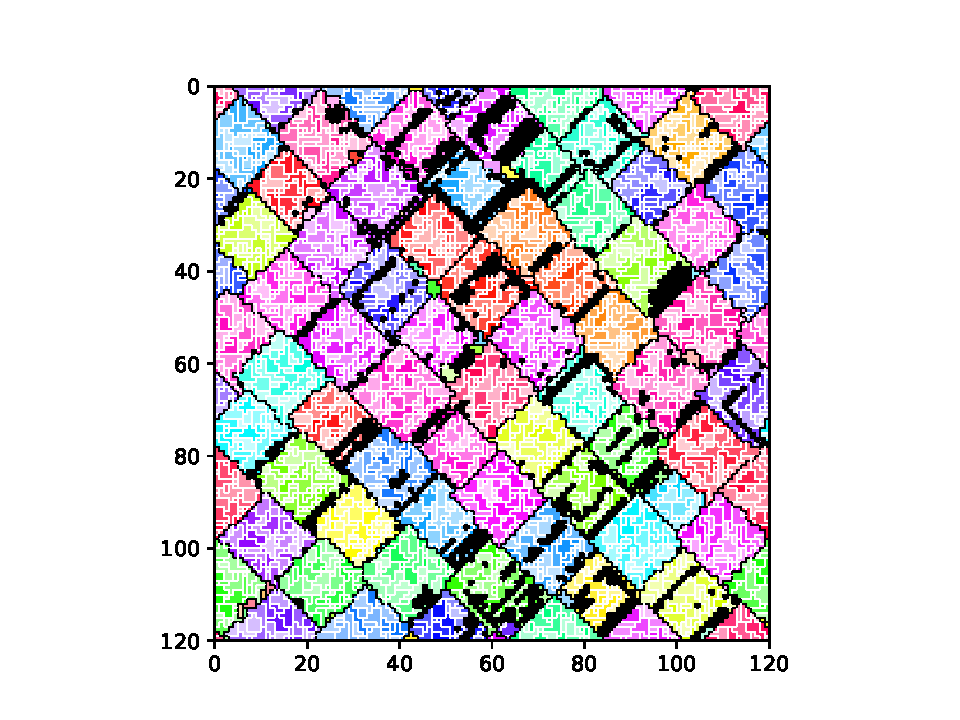
\includegraphics[width=\columnwidth,trim={2.5cm 0.5cm 2.5cm 1cm},clip]{img/ChannelMap_1008_update19500000}
  \caption{Mean $P_2 = 1.0$; gen. 25,841\\~}
  \label{fig:ChannelMap_1008}
\end{subfigure}

\caption{
End state of same-channel signaling networks in replicates where cell- (\ref{fig:ChannelMap_1022}), first- (\ref{fig:ChannelMap_1041}), and second-level (\ref{fig:ChannelMap_1008}) individuality dominated.
(Cell-level individuals are single cells that retain collected resource exclusively for their own use, first-level individuals are level-one same-channel multi-cellular networks that primarily assign collected resource for collective use among level-one channel mates, and second-level individuals are level-two same-channel multi-cellular networks that primarily assign collected resource for collective use among level-two channel mates.)
Level-one channels are coded by color saturation and level-two channels are coded by color hue.
A single cell-like organism occupies each grid tile except for black tiles, which are empty.
}
\label{fig:outcome_grids}
\end{center}
\end{figure*}


\begin{figure*}%[!htbp]
\begin{center}

\begin{subfigure}[b]{0.33\columnwidth}
  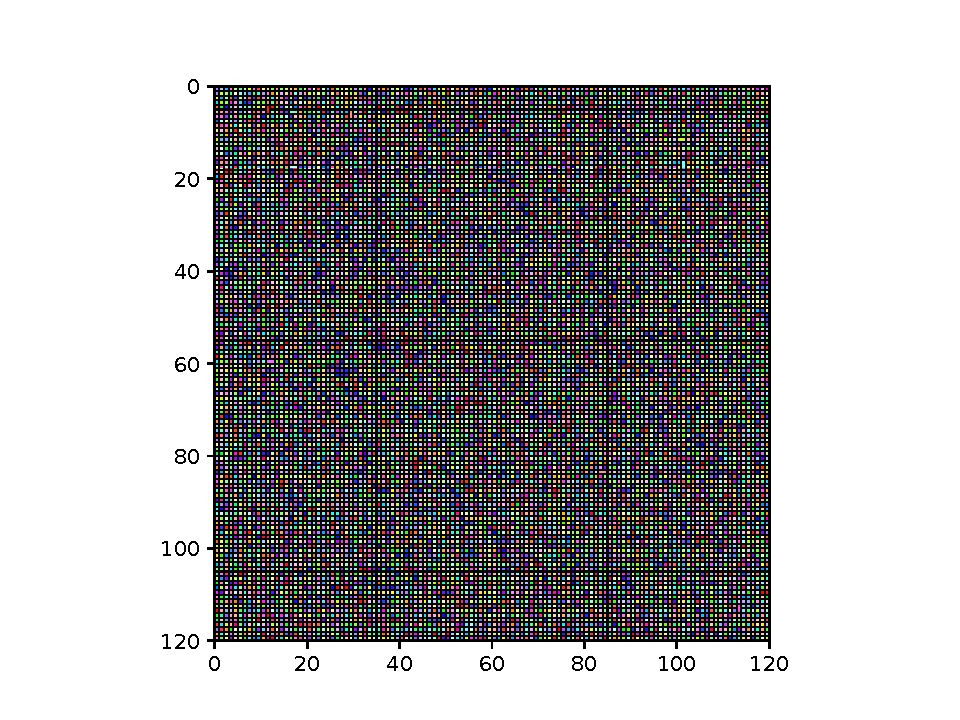
\includegraphics[width=\columnwidth,trim={2.5cm 0.5cm 2.5cm 1cm},clip]{img/ChannelMap_1007_update0}
  \vspace{-5ex}
  \caption{Update 0; cell gen. 0}
  \label{fig:ChannelMap_1007_update0}
\end{subfigure}%
\begin{subfigure}[b]{0.33\columnwidth}
  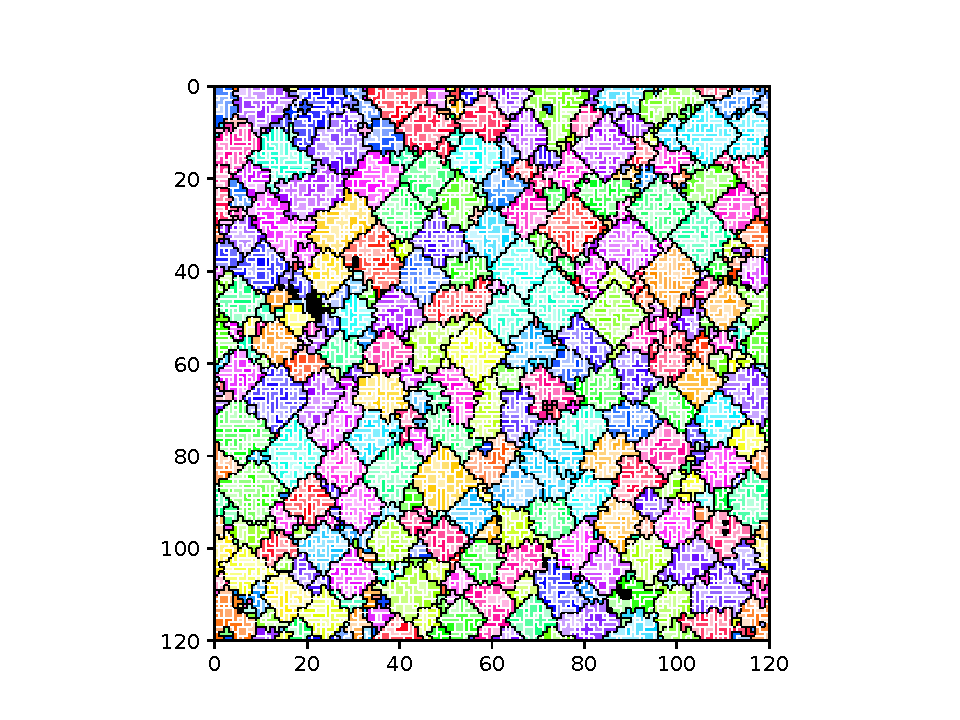
\includegraphics[width=\columnwidth,trim={2.5cm 0.5cm 2.5cm 1cm},clip]{img/ChannelMap_1007_update55520}
  \vspace{-5ex}
  \caption{Update 55520; cell gen. 103}
  \label{fig:ChannelMap_1007_update55520}
\end{subfigure}%
\begin{subfigure}[b]{0.33\columnwidth}
  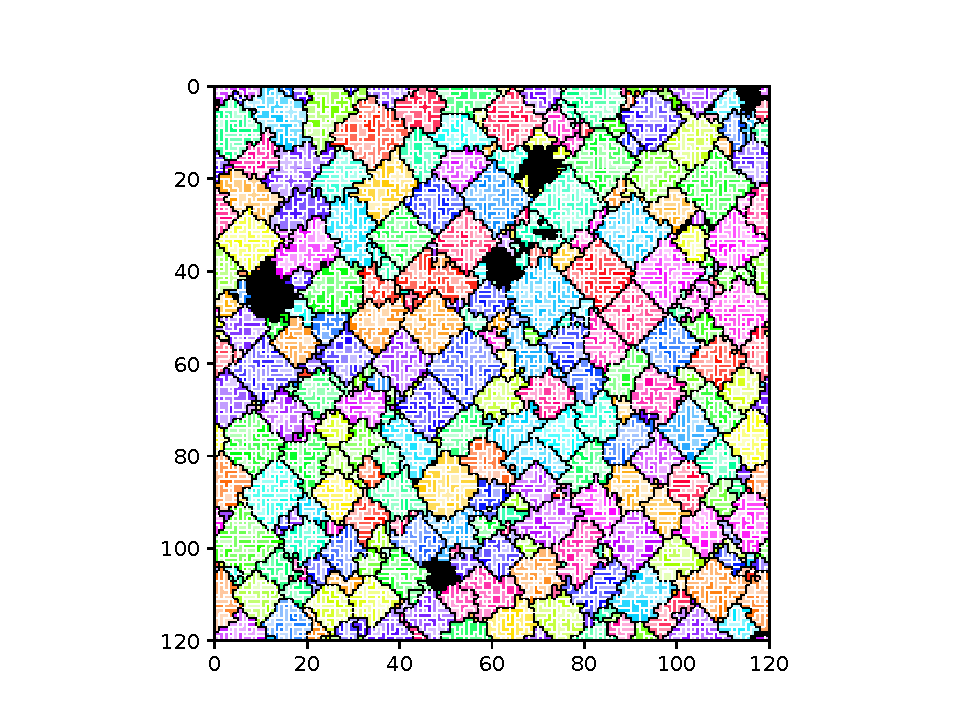
\includegraphics[width=\columnwidth,trim={2.5cm 0.5cm 2.5cm 1cm},clip]{img/ChannelMap_1007_update277600}
  \vspace{-5ex}
  \caption{Update 277600; cell gen. 563}
  \label{fig:ChannelMap_1007_update277600}
\end{subfigure}

\begin{subfigure}[b]{0.33\columnwidth}
  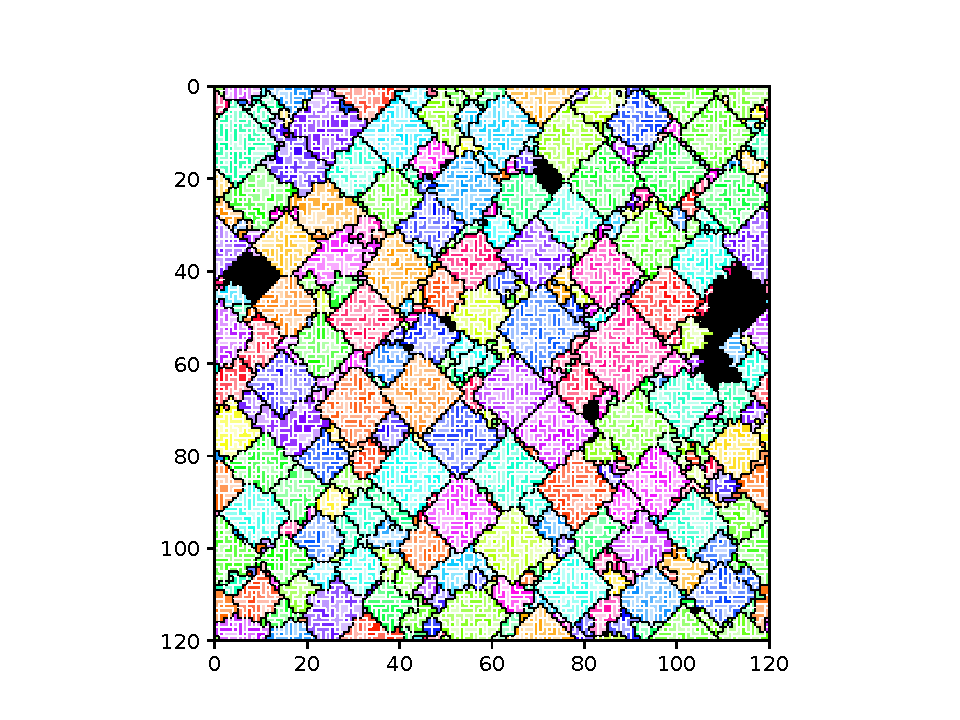
\includegraphics[width=\columnwidth,trim={2.5cm 0.5cm 2.5cm 1cm},clip]{img/ChannelMap_1007_update500000}
  \vspace{-5ex}
  \caption{Update 500000; cell gen. 1072}
  \label{fig:ChannelMap_1007_update500000}
\end{subfigure}%
\begin{subfigure}[b]{0.33\columnwidth}
  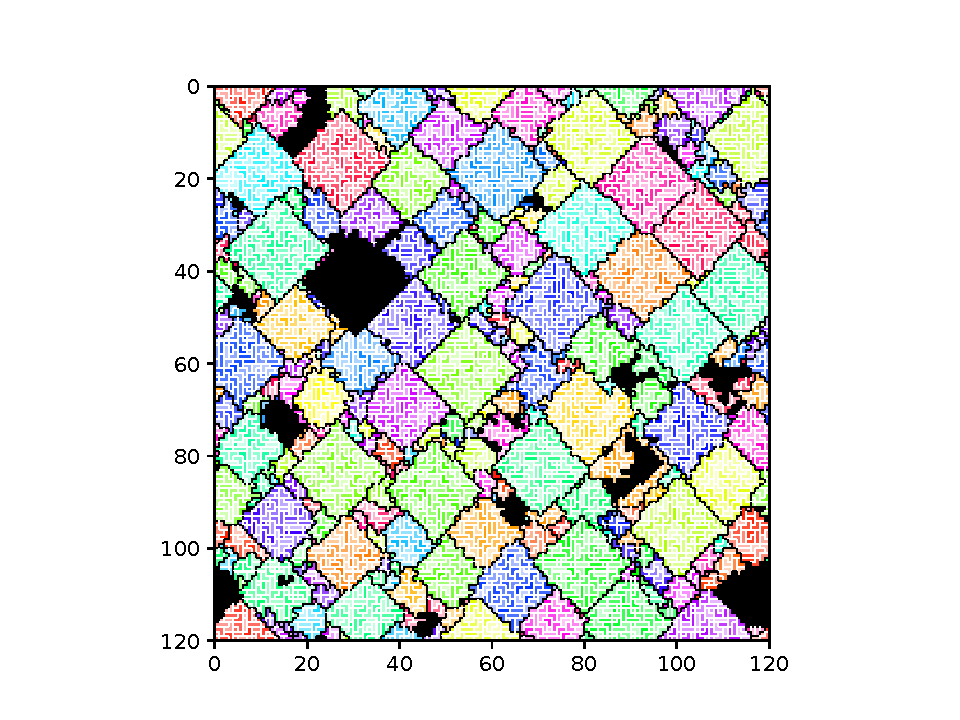
\includegraphics[width=\columnwidth,trim={2.5cm 0.5cm 2.5cm 1cm},clip]{img/ChannelMap_1007_update1000000}
  \vspace{-5ex}
  \caption{Update 1000000; cell gen. 2405}
  \label{fig:ChannelMap_1007_update1000000}
\end{subfigure}%
\begin{subfigure}[b]{0.33\columnwidth}
  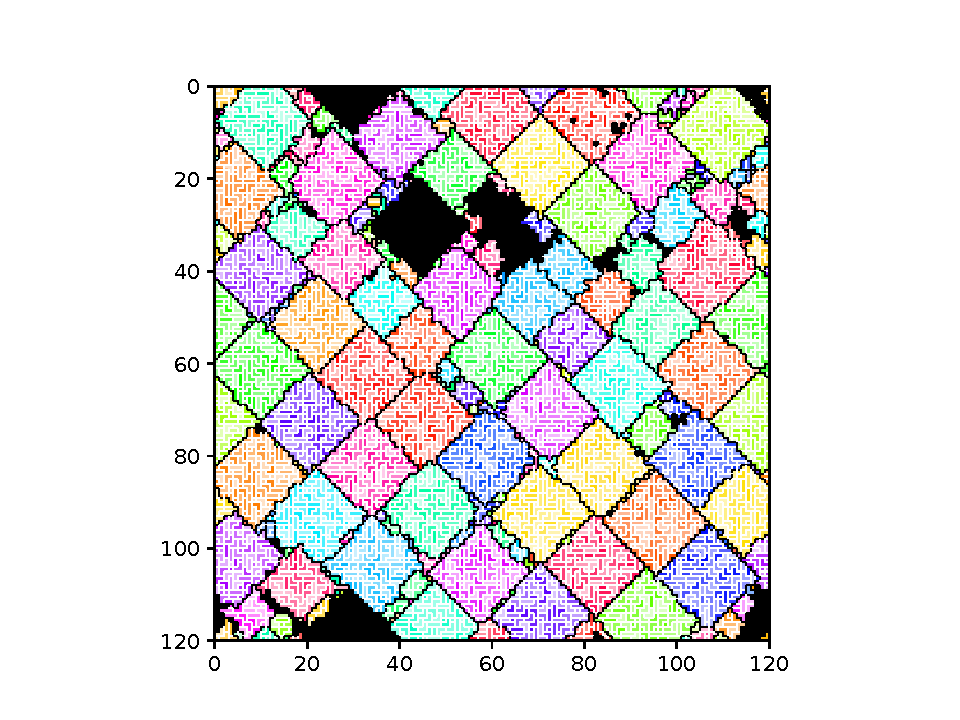
\includegraphics[width=\columnwidth,trim={2.5cm 0.5cm 2.5cm 1cm},clip]{img/ChannelMap_1007_update2000000}
  \vspace{-5ex}
  \caption{Update 2000000; cell gen. 4974}
  \label{fig:ChannelMap_1007_update2000000}
\end{subfigure}

\caption{
Progression of same-channel level-one and level-two signaling networks states in an evolutionary run where level-two resource sharing evolved.
Level-one channels are coded by color saturation and level-two channels are coded by color hue.
A single cell-like organism occupies each grid tile except for black tiles, which are empty.
Level-one same-channel groups appear as uniformly-colored clumps, bounded by a white border.
Level-two same-channel groups appear as same-hue amalgamations of level-one groups, bounded by a black border.
}
\label{fig:grid_progression}
\end{center}
\end{figure*}


\begin{figure}[t]
\begin{center}

\begin{subfigure}[b]{\columnwidth}
  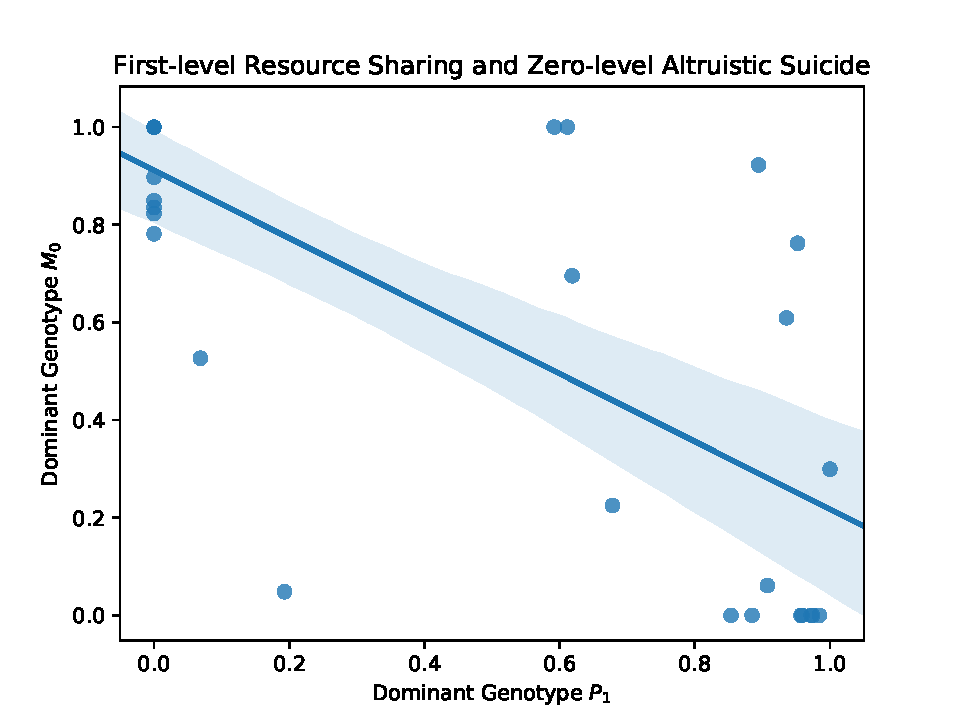
\includegraphics[width=\columnwidth]{img/champion_res_pool1_vs_champion_damage_suicide0}
  \label{fig:champion_res_pool1_vs_champion_damage_suicide0}
\end{subfigure}

\begin{subfigure}[b]{\columnwidth}
  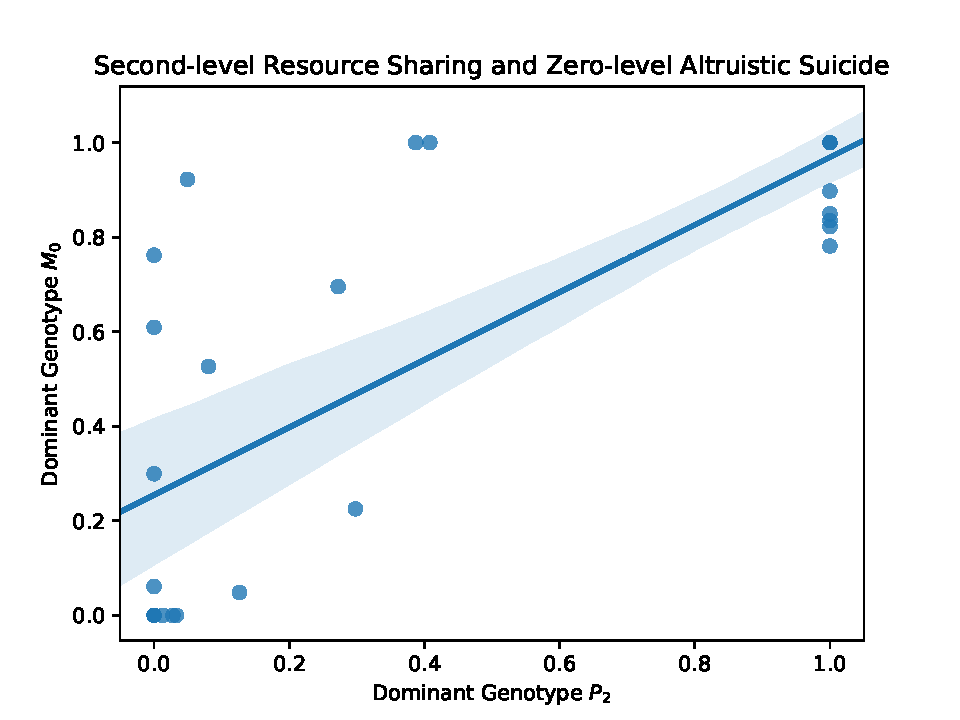
\includegraphics[width=\columnwidth]{img/champion_res_pool2_vs_champion_damage_suicide0}
  \label{fig:champion_res_pool2_vs_champion_damage_suicide0}
\end{subfigure}

\caption{
TODO
}
\label{fig:damage_suicide}
\end{center}
\end{figure}


\begin{figure}[t]
\begin{center}

\begin{subfigure}[b]{\columnwidth}
  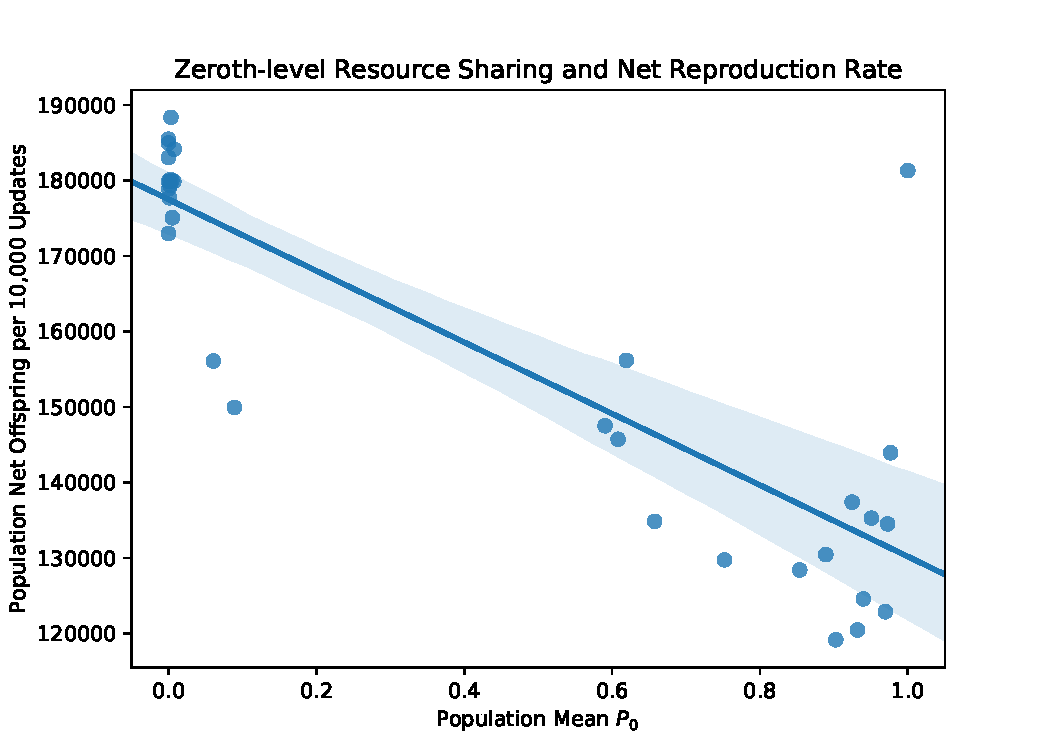
\includegraphics[width=\columnwidth]{img/mean_res_pool1_vs_net_reproduction}
  \caption{
  Correlation plot of population mean $P_1$ and population net reproduction rate.
  }
  \label{fig:mean_res_pool1_vs_net_reproduction}
\end{subfigure}

\begin{subfigure}[b]{\columnwidth}
  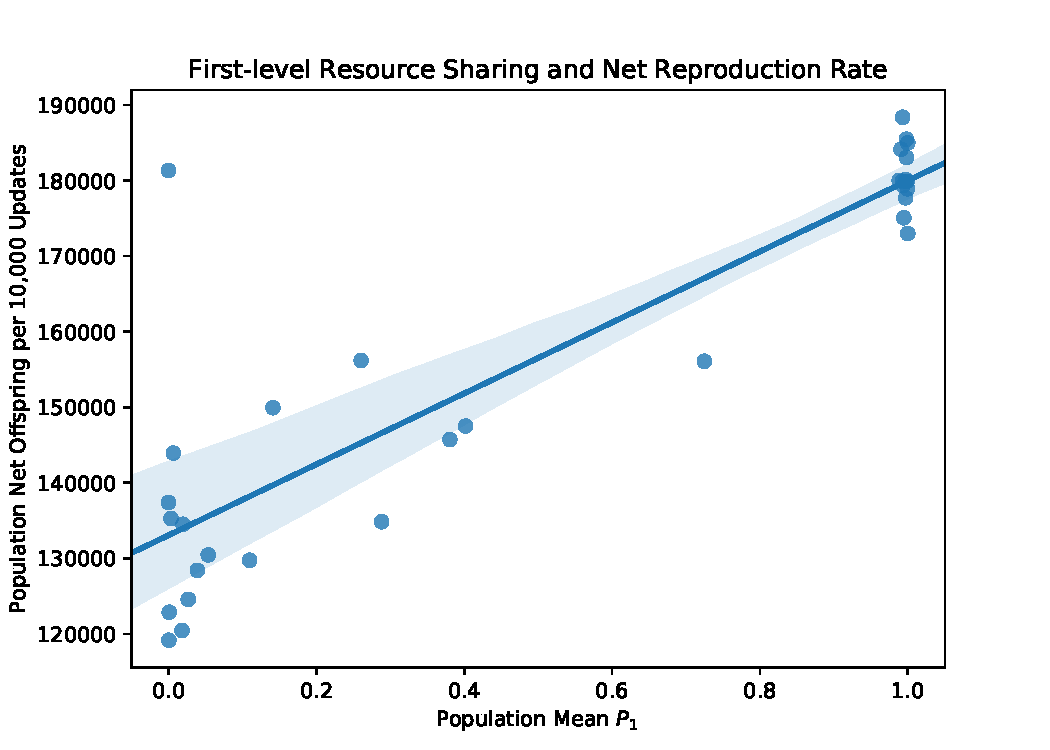
\includegraphics[width=\columnwidth]{img/mean_res_pool2_vs_net_reproduction}
  \caption{
  Correlation plot of population mean $P_2$ and population net reproduction rate.
  }
  \label{fig:mean_res_pool2_vs_net_reproduction}
\end{subfigure}

\caption{
Plot of population mean resource caching strategies and population net reproduction rate.
}
\label{fig:net_reproduction}
\end{center}
\end{figure}


\begin{figure}[t]
\begin{center}

\begin{subfigure}[b]{\columnwidth}
  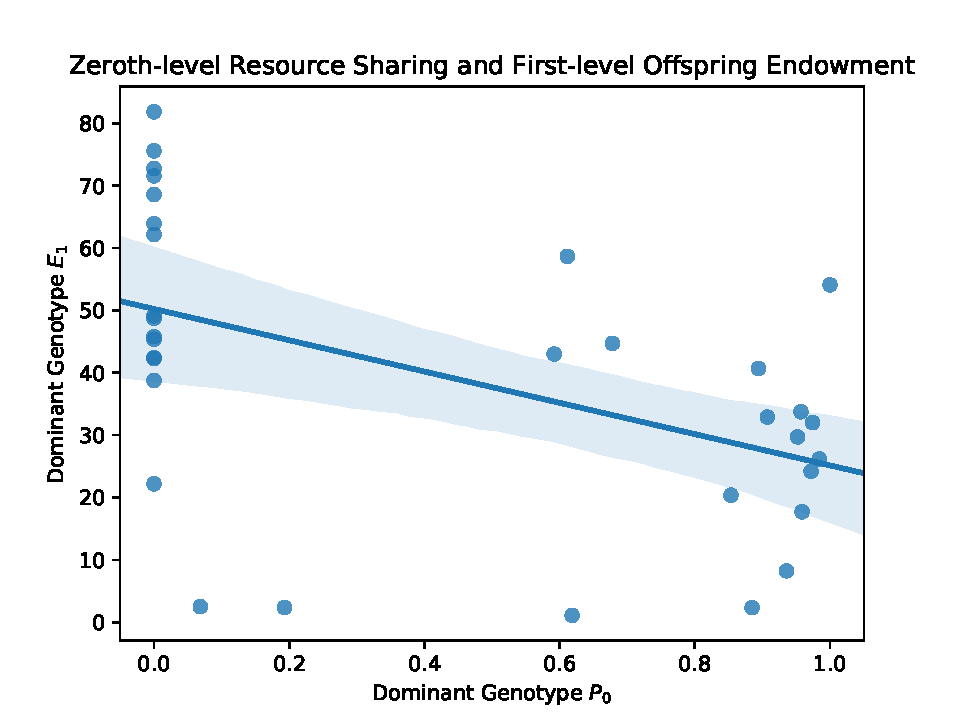
\includegraphics[width=\columnwidth]{img/champion_res_pool1_vs_champion_endowment2}
  \caption{
  Correlation plot of dominant genotype $P_1$ and dominant genotype $E_2$.
  }
  \label{fig:champion_res_pool1_vs_champion_endowment2}
\end{subfigure}

\begin{subfigure}[b]{\columnwidth}
  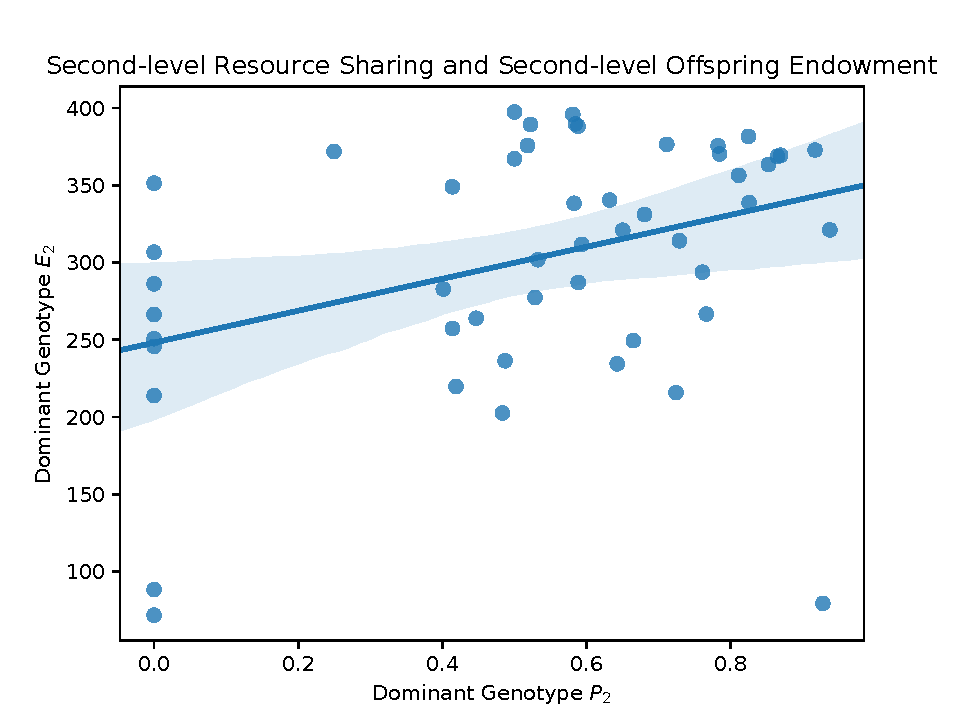
\includegraphics[width=\columnwidth]{img/champion_res_pool2_vs_champion_endowment2}
  \caption{
  Correlation plot of dominant genotype $P_2$ and dominant genotype $E_2$.
  }
  \label{fig:champion_res_pool2_vs_champion_endowment2}
\end{subfigure}

\caption{
Plots of dominant resource caching strategies and dominant propagule endowment strategies.
A bootstrapped 95\% confidence interval for the fit is shaded.
}
\label{fig:endowment}
\end{center}
\end{figure}


Cell-, zeroth-, and first-level individuals were all observed at the conclusion of different runs of our evolutionary simulation (mean generation 22,016; $s=3,119$).
The criteria used to discern these outcomes are described below.
Figure \ref{fig:outcome_grids} shows the level-zero and level-one signaling networks at the end of runs where cell-, zeroth-, and first-level individuality evolved, respectively.
Figure \ref{fig:grid_progression} shows a time series of signaling network snapshots in an evolutionary run where first-level individuality evolved.
Cell-level individuals appear to form with comparatively large level-zero signaling networks that are arranged into amorphous level-one signaling networks.
Zeroth-level individuals appear to form elongated cigar-shaped level one amalgamations of diverse level-zero networks.
First-level individuals appear to form highly regular diamond-shaped level one amalgamations of diverse level zero networks.

Figure \ref{fig:genotypes} describes predominant genotypes observed at the end of our evolutionary simulations.
With a single exception, nearly all evolved genotypes had $A_1$ fixed at or very near $1.0$ (i.e. population mean $A_1 \geq 0.993$).
So, reproduction over cells sharing the same level-one channel was near-universally avoided;
genotypes evolved so that cell-level organisms declined to reproduce when they were located at the interior of level one same-channel signaling networks.

However, a variety of resource-caching strategies evolved.
Most-abundant genotypes at the end of evolutionary runs included strategies where resource was primarily cached in an organism's individual stockpile (i.e. $P_{c} > P_0, P_1$), strategies where resource was primarily cached in an organism's level-zero signaling network's pool (i.e. $P_0 > P_{c}, P_1$), and strategies where resource was primarily cached in an organism's level-one signaling network's pool (i.e. $P_1 > P_{c}, P_0$).
Among 33 trials, selfish cell-level hoarders dominated at the end of two replicates, level-zero resource-sharing dominated in 16 replicates, and level-one resource sharing dominated in 15 replicates.

Given the near-ubiquitous nature of cooperation with regard to reproductive division of labor at the level one same-channel signaling network, it was on this basis of resource caching strategy that we drew distinctions between cell-, zeroth-, and first-level individuality.
(The single predominant genotype with $A_1 = 0.91$ had $P_0 = 1.0$, so was not sharing resource on the level one same-channel resource pool).
% @CAO: I'm not sure where this final parenthetical came from.  I take it this is the single "selfish" individual in the second example above?
% @MAM: Exactly.

Next, we wanted to compare cell-, zeroth-, and first-level individuals to determine which genotype was the most fit in the DISHTINY environment.
We ran ecological competitions between the the dominant genotypes from the run with greatest mean $P_{c}$, the run with greatest mean $P_0$, and the run with greatest mean $P_1$.
In 22 out of 191 trials performed fixation was reached by update 1.5 million.  The cell-level individuality genotype dominated in one trial, the zeroth-level individuality genotype dominated in 12 trials, and the first-level individuality genotype dominated in 178 trials.
These results show that in the absence of mutation, first-level individuals tend to exhibit greater fitness than zeroth- and cell-th level individuals ($p < 0.0001$; RR 2.8; two-tailed exact test).

In ecological competition, however, higher-level individuals likely benefited from elimination of somatic mutation.
To assess the relative fitness of zeroth- and first-level individuals without mutation disabled, we examined the relationship between zeroth/first-level resource pooling and the rate of cellular reproduction at the end of each of the 33 replicate evolutionary trials performed.
We observed a significant negative correlation between mean $P_0$ and cellular reproduction rate ($p < 0.0001$; bootstrap test; Figure \ref{fig:mean_res_pool1_vs_net_reproduction}) and a significant positive correlation between mean $P_1$ and cellular reproduction rate ($p < 0.0001$; bootstrap test; Figure \ref{fig:mean_res_pool2_vs_net_reproduction}).
This result suggests that first-level individuals tend to collect resource more effectively than zeroth-level individuals.
We did not test correlation between $P_{c}$ and reproduction rate due to the small number of outcomes where cell-level individuality.

With the viability of cell-, zeroth-, and first-level individuality in the DISHTINY environment --- and the greater relative fitness of first-level individuality --- established, we were also interested in probing the strategies employed by cell-, zeroth-, and first-level individuals beyond resource caching and reproductive deferment.
To assess whether higher-level individuals employed apoptosis to mitigate somatic mutation, we examined the relationship between zeroth/first-level resource pooling and cell-level apoptosis at the conclusion of our 33 replicate evolutionary trials.
We observed a significant negative correlation between dominant genotype $P_0$ and $M_{c}$ ($p < 0.0001$; bootstrap test; Figure \ref{fig:champion_res_pool1_vs_champion_damage_suicide0}) and a significant positive correlation between dominant genotype $P_1$ and $M_{c}$ ($p < 0.0001$; bootstrap test; Figure \ref{fig:champion_res_pool2_vs_champion_damage_suicide0}).
Notably, no genotype encoding first-level individuality was observed with $M_{c} < 0.5$.
This result suggests that first-level individuals, in particular, relied on apoptosis to mitigate somatic mutation, perhaps due to their much larger scale compared to cell- and zeroth-level individuals.

To assess whether higher-level individuals provided larger resource endowments to their propagules (offspring sharing neither the level zero nor the level one channel ID with the parent), we examined the relationship between zeroth/first-level resource pooling and dominant genotype first-level propagule endowment at the conclusion of our 33 replicate evolutionary trials.
We observed a significant negative correlation between dominant genotype $P_0$ and $E_1$ ($p < 0.001$; bootstrap test; Figure \ref{fig:champion_res_pool1_vs_champion_endowment2}) and a significant positive correlation between dominant genotype $P_1$ and $E_1$ ($p <  0.0001$; bootstrap test; Figure \ref{fig:champion_res_pool2_vs_champion_endowment2}).
First-level individuals might provide larger endowments to propagules simply due to a greater capacity to collect resource or perhaps because of stronger selection for well-endowed offspring when competing against other first-level individuals.
